\documentclass[a4paper,10pt,twocolumn]{article}
\title{\textbf{\underline{REPORT: Logistic Regression}}}
\usepackage[left=2cm, right=2cm, top=1.5cm]{geometry}
\usepackage{xcolor}
\usepackage{ragged2e}
\usepackage{lipsum,multicol}
\usepackage{graphicx}
\usepackage{subfig}
\usepackage{amsmath, amsfonts}
\usepackage{times}
\date{}
\author{}
\begin{document}
\maketitle
%===================================================================================================================%
\section*{\textcolor{blue}{1. Introduction:}}
In this report, we try to analyse the performance (accuracy, fscore, recall and precision) of a logistic regression that we built using NumPy. The implementation of this network is similar to that of sklearn and the whole code has been written in a completely modularized fashion.

\section*{\textcolor{blue}{2. Data Preprocessing:}}
The dataset contained 1372 data points, each containing 4 input features (representing banknote features) and one binary target variable (representing if the note is authentic or not). In the preprocessing stage, all features were standardized/normalized and randomly split into \textit{train\_set}, \textit{test\_set} and \textit{validation\_set}(70-20-10 split ratio).

\section*{\textcolor{blue}{3. Non-Linear function:}}
\begin{itemize}
\item{sigmoid: $y$ = $\frac{1}{1 + e^{-x}}$}
\end{itemize}

\section*{\textcolor{blue}{4. Loss function:}}
\begin{itemize}
\item{$L_n = -t_nlog(y_n)-(1-t_n)log(1-y_n)$} 
\end{itemize}

\section*{\textcolor{blue}{5. Model Architecture:}}
The predictions for the whole training set were made according to the following formula: $\sigma(\widetilde{W}^T \widetilde{X})$ where $\widetilde{X}$ represents the input features padded with ones to accomodate the bias term and $\sigma$ represents the sigmoid function.




\section*{\textcolor{blue}{6. Conclusion:}}
\begin{itemize}
\item{In general, a three layer network performs better than a two layer network. Adding more layers/more neurons to the hidden layers provides more trainable parameters which help the network to fit the model in a better way. But the drawback of adding multiple layers/mulitple neurons is that, the model requires more iterations to train. In this case, there is a higher chance that the model might overfit the data, and hence giving a low testing accuracy.}
\item{A lower learning rate requires more iterations to converge, but conversely, using a higher learning rate might lead to fluctuation in the loss/exploding gradient.}
\item{Different initialization of weights leads to convergence of the model at different local minima (initializations mentioned above).}
\item{Different activation functions for the hidden layers provides drastically varying results. We	 have used ReLU (Rectified Linear) which is by and the far, the de-facto standard activation used for hidden layers. Other activations like tanh or sigmoid gave very low accuracy as compared to that of ReLU. ReLU suffers from the \emph{dying neuron problem}, in which the output of a neuron might be 0 for most of the training (i.e. that neuron is not contributing to the network), and hence we tried using leaky-ReLU, but the accuracy was found to more or less the same.}
\end{itemize}
[results on next page]

\newpage
\onecolumn
\section*{\textcolor{blue}{7. Results:}}
\begin{figure}[h!]
\centering
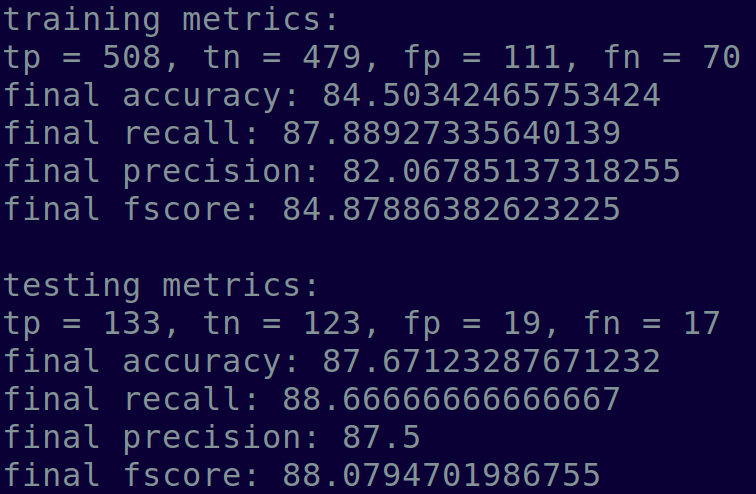
\includegraphics[scale=1.0, width=5cm]{Fig1.png}
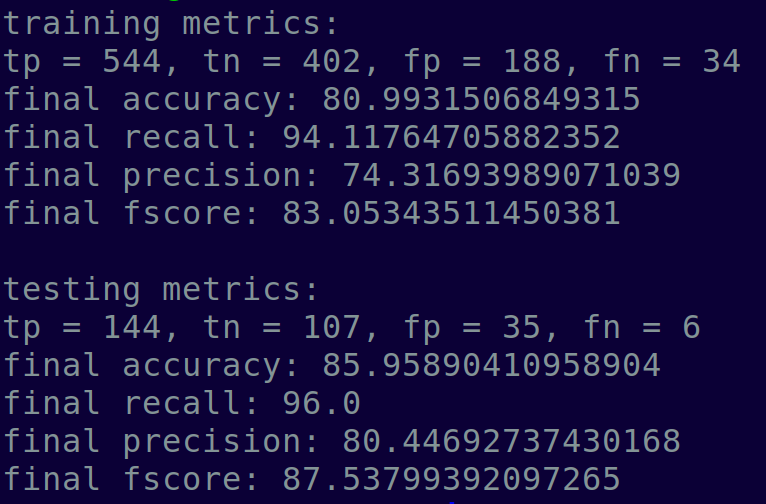
\includegraphics[scale=1.0, width=5cm]{Fig2.png}
\caption*{2-Layer NN using uniform distribution}
\end{figure}

\begin{figure}[h!]
\centering
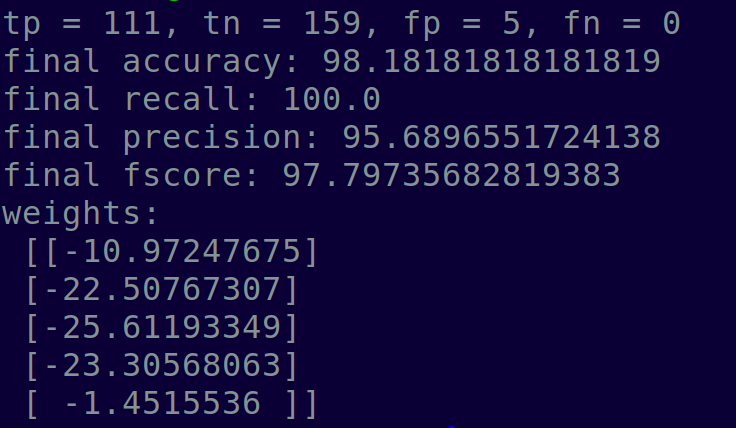
\includegraphics[scale=1.0, width=5cm]{Fig3.png}
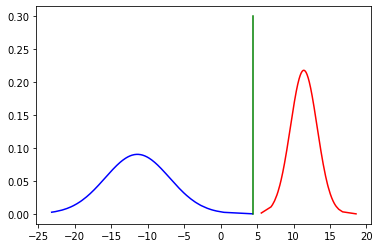
\includegraphics[scale=1.0, width=5cm]{Fig4.png}
\caption*{3-Layer NN using uniform distirbution}
\end{figure}

\begin{figure}[h!]
\centering
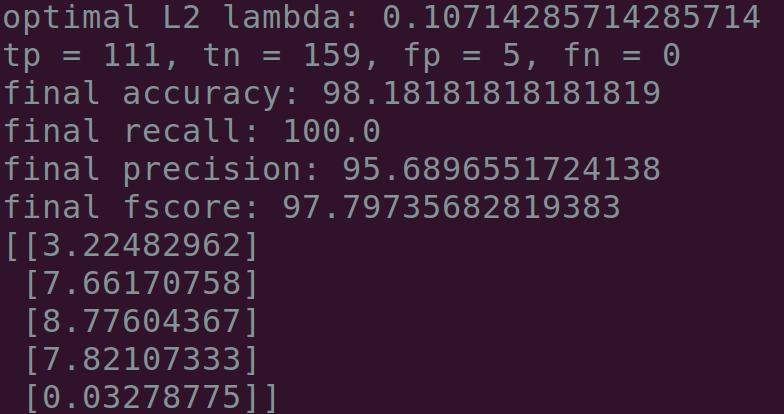
\includegraphics[scale=1.0, width=5cm]{Fig5.png}
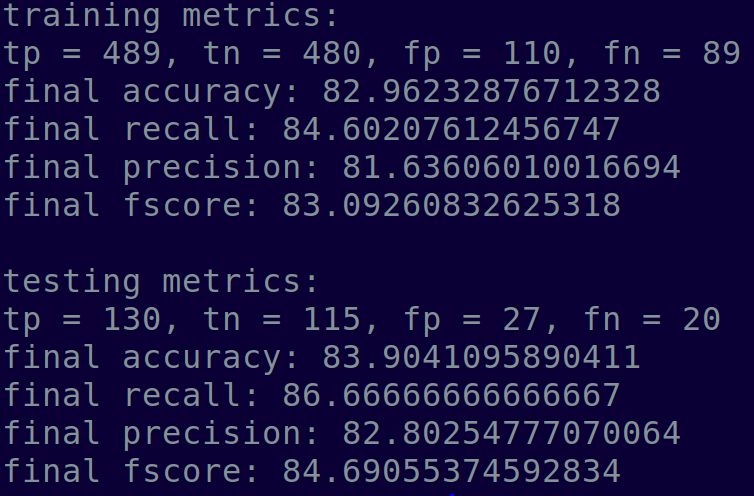
\includegraphics[scale=1.0, width=5cm]{Fig6.png}
\caption*{2-Layer NN using normal distirbution}
\end{figure}

\begin{figure}[h!]
\centering
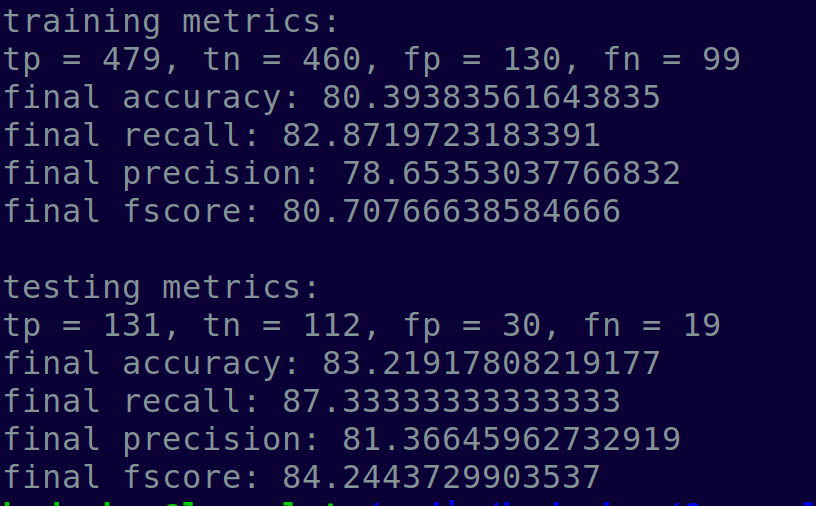
\includegraphics[scale=1.0, width=5cm]{Fig7.png}
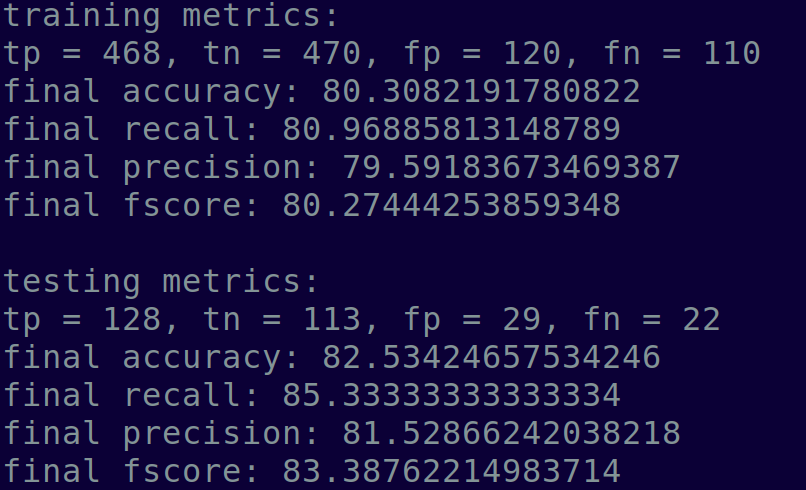
\includegraphics[scale=1.0, width=5cm]{Fig8.png}
\caption*{3-Layer NN using normal distirbution}
\end{figure}
%=================================================================================================================%
\end{document}
